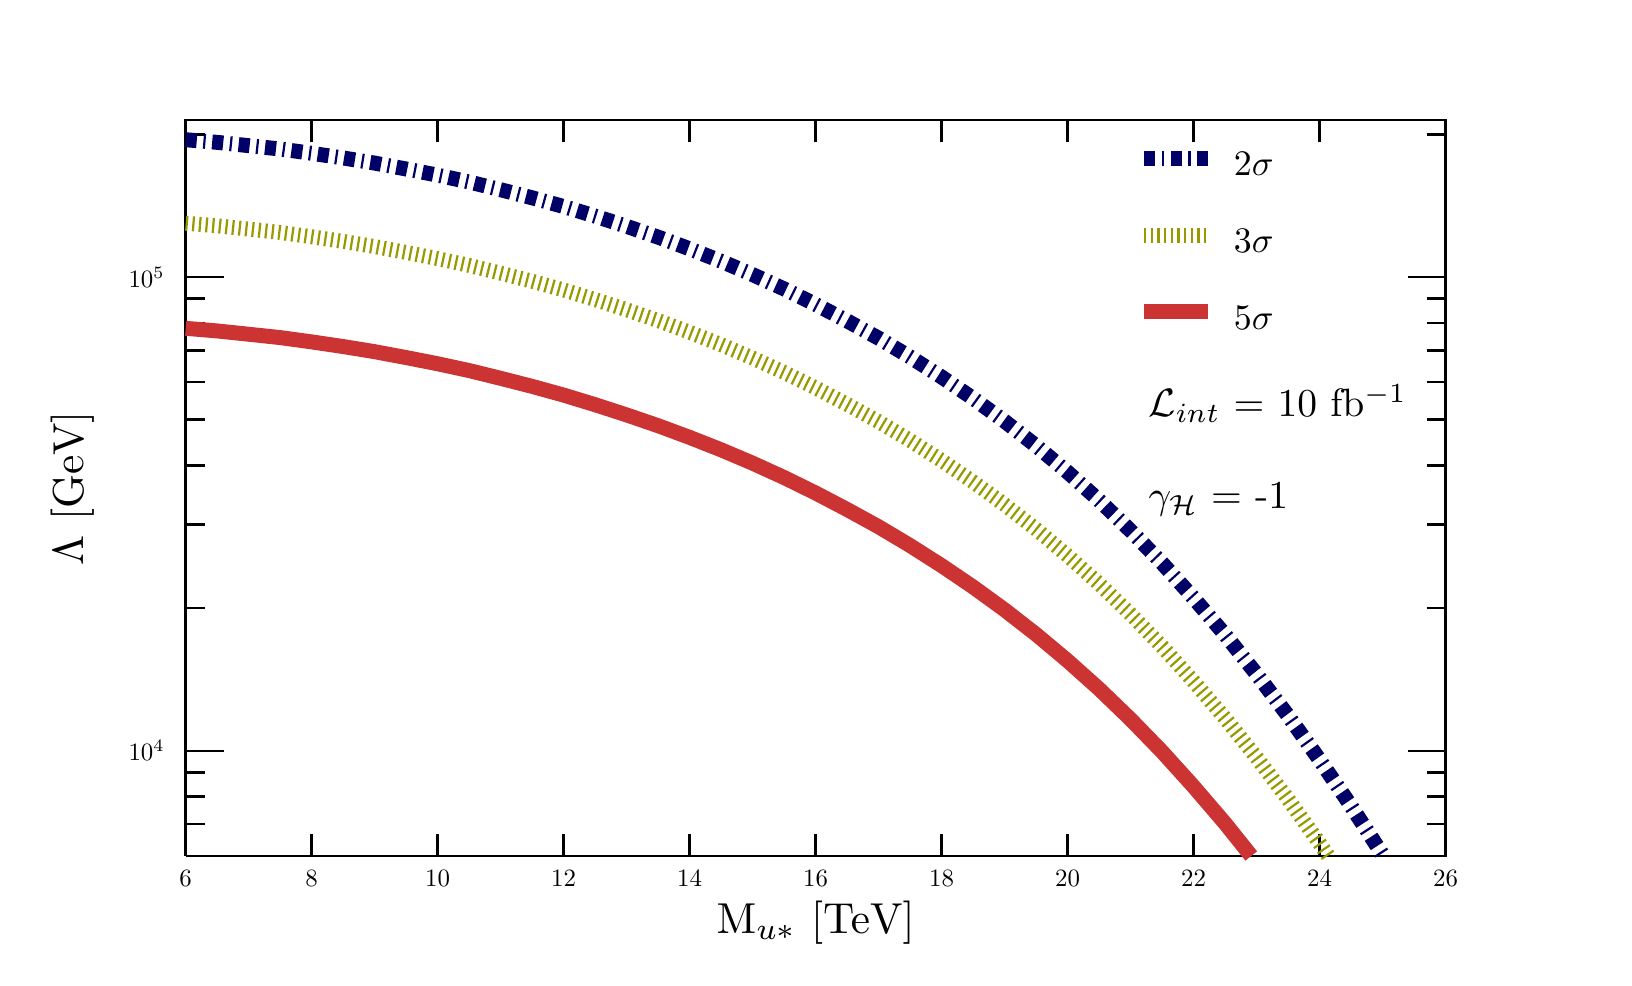
\begin{tikzpicture}
\pgfdeclareplotmark{cross} {
\pgfpathmoveto{\pgfpoint{-0.3\pgfplotmarksize}{\pgfplotmarksize}}
\pgfpathlineto{\pgfpoint{+0.3\pgfplotmarksize}{\pgfplotmarksize}}
\pgfpathlineto{\pgfpoint{+0.3\pgfplotmarksize}{0.3\pgfplotmarksize}}
\pgfpathlineto{\pgfpoint{+1\pgfplotmarksize}{0.3\pgfplotmarksize}}
\pgfpathlineto{\pgfpoint{+1\pgfplotmarksize}{-0.3\pgfplotmarksize}}
\pgfpathlineto{\pgfpoint{+0.3\pgfplotmarksize}{-0.3\pgfplotmarksize}}
\pgfpathlineto{\pgfpoint{+0.3\pgfplotmarksize}{-1.\pgfplotmarksize}}
\pgfpathlineto{\pgfpoint{-0.3\pgfplotmarksize}{-1.\pgfplotmarksize}}
\pgfpathlineto{\pgfpoint{-0.3\pgfplotmarksize}{-0.3\pgfplotmarksize}}
\pgfpathlineto{\pgfpoint{-1.\pgfplotmarksize}{-0.3\pgfplotmarksize}}
\pgfpathlineto{\pgfpoint{-1.\pgfplotmarksize}{0.3\pgfplotmarksize}}
\pgfpathlineto{\pgfpoint{-0.3\pgfplotmarksize}{0.3\pgfplotmarksize}}
\pgfpathclose
\pgfusepathqstroke
}
\pgfdeclareplotmark{cross*} {
\pgfpathmoveto{\pgfpoint{-0.3\pgfplotmarksize}{\pgfplotmarksize}}
\pgfpathlineto{\pgfpoint{+0.3\pgfplotmarksize}{\pgfplotmarksize}}
\pgfpathlineto{\pgfpoint{+0.3\pgfplotmarksize}{0.3\pgfplotmarksize}}
\pgfpathlineto{\pgfpoint{+1\pgfplotmarksize}{0.3\pgfplotmarksize}}
\pgfpathlineto{\pgfpoint{+1\pgfplotmarksize}{-0.3\pgfplotmarksize}}
\pgfpathlineto{\pgfpoint{+0.3\pgfplotmarksize}{-0.3\pgfplotmarksize}}
\pgfpathlineto{\pgfpoint{+0.3\pgfplotmarksize}{-1.\pgfplotmarksize}}
\pgfpathlineto{\pgfpoint{-0.3\pgfplotmarksize}{-1.\pgfplotmarksize}}
\pgfpathlineto{\pgfpoint{-0.3\pgfplotmarksize}{-0.3\pgfplotmarksize}}
\pgfpathlineto{\pgfpoint{-1.\pgfplotmarksize}{-0.3\pgfplotmarksize}}
\pgfpathlineto{\pgfpoint{-1.\pgfplotmarksize}{0.3\pgfplotmarksize}}
\pgfpathlineto{\pgfpoint{-0.3\pgfplotmarksize}{0.3\pgfplotmarksize}}
\pgfpathclose
\pgfusepathqfillstroke
}
\pgfdeclareplotmark{newstar} {
\pgfpathmoveto{\pgfqpoint{0pt}{\pgfplotmarksize}}
\pgfpathlineto{\pgfqpointpolar{44}{0.5\pgfplotmarksize}}
\pgfpathlineto{\pgfqpointpolar{18}{\pgfplotmarksize}}
\pgfpathlineto{\pgfqpointpolar{-20}{0.5\pgfplotmarksize}}
\pgfpathlineto{\pgfqpointpolar{-54}{\pgfplotmarksize}}
\pgfpathlineto{\pgfqpointpolar{-90}{0.5\pgfplotmarksize}}
\pgfpathlineto{\pgfqpointpolar{234}{\pgfplotmarksize}}
\pgfpathlineto{\pgfqpointpolar{198}{0.5\pgfplotmarksize}}
\pgfpathlineto{\pgfqpointpolar{162}{\pgfplotmarksize}}
\pgfpathlineto{\pgfqpointpolar{134}{0.5\pgfplotmarksize}}
\pgfpathclose
\pgfusepathqstroke
}
\pgfdeclareplotmark{newstar*} {
\pgfpathmoveto{\pgfqpoint{0pt}{\pgfplotmarksize}}
\pgfpathlineto{\pgfqpointpolar{44}{0.5\pgfplotmarksize}}
\pgfpathlineto{\pgfqpointpolar{18}{\pgfplotmarksize}}
\pgfpathlineto{\pgfqpointpolar{-20}{0.5\pgfplotmarksize}}
\pgfpathlineto{\pgfqpointpolar{-54}{\pgfplotmarksize}}
\pgfpathlineto{\pgfqpointpolar{-90}{0.5\pgfplotmarksize}}
\pgfpathlineto{\pgfqpointpolar{234}{\pgfplotmarksize}}
\pgfpathlineto{\pgfqpointpolar{198}{0.5\pgfplotmarksize}}
\pgfpathlineto{\pgfqpointpolar{162}{\pgfplotmarksize}}
\pgfpathlineto{\pgfqpointpolar{134}{0.5\pgfplotmarksize}}
\pgfpathclose
\pgfusepathqfillstroke
}
\definecolor{c}{rgb}{1,1,1};
\draw [color=c, fill=c] (0,0) rectangle (20,11.6806);
\draw [color=c, fill=c] (2,1.16806) rectangle (18,10.5125);
\definecolor{c}{rgb}{0,0,0};
\draw [c,line width=0.9] (2,1.16806) -- (2,10.5125) -- (18,10.5125) -- (18,1.16806) -- (2,1.16806);
\definecolor{c}{rgb}{1,1,1};
\draw [color=c, fill=c] (2,1.16806) rectangle (18,10.5125);
\definecolor{c}{rgb}{0,0,0};
\draw [c,line width=0.9] (2,1.16806) -- (2,10.5125) -- (18,10.5125) -- (18,1.16806) -- (2,1.16806);
\draw [c,line width=0.9] (2,1.16806) -- (18,1.16806);
\draw (10,0.327056) node[scale=1.56475, color=c, rotate=0]{M$_{u*}$ [TeV]};
\draw [c,line width=0.9] (2,1.44839) -- (2,1.16806);
\draw [c,line width=0.9] (3.6,1.44839) -- (3.6,1.16806);
\draw [c,line width=0.9] (5.2,1.44839) -- (5.2,1.16806);
\draw [c,line width=0.9] (6.8,1.44839) -- (6.8,1.16806);
\draw [c,line width=0.9] (8.4,1.44839) -- (8.4,1.16806);
\draw [c,line width=0.9] (10,1.44839) -- (10,1.16806);
\draw [c,line width=0.9] (11.6,1.44839) -- (11.6,1.16806);
\draw [c,line width=0.9] (13.2,1.44839) -- (13.2,1.16806);
\draw [c,line width=0.9] (14.8,1.44839) -- (14.8,1.16806);
\draw [c,line width=0.9] (16.4,1.44839) -- (16.4,1.16806);
\draw [c,line width=0.9] (18,1.44839) -- (18,1.16806);
\draw [anchor=base] (2,0.782598) node[scale=0.900036, color=c, rotate=0]{6};
\draw [anchor=base] (3.6,0.782598) node[scale=0.900036, color=c, rotate=0]{8};
\draw [anchor=base] (5.2,0.782598) node[scale=0.900036, color=c, rotate=0]{10};
\draw [anchor=base] (6.8,0.782598) node[scale=0.900036, color=c, rotate=0]{12};
\draw [anchor=base] (8.4,0.782598) node[scale=0.900036, color=c, rotate=0]{14};
\draw [anchor=base] (10,0.782598) node[scale=0.900036, color=c, rotate=0]{16};
\draw [anchor=base] (11.6,0.782598) node[scale=0.900036, color=c, rotate=0]{18};
\draw [anchor=base] (13.2,0.782598) node[scale=0.900036, color=c, rotate=0]{20};
\draw [anchor=base] (14.8,0.782598) node[scale=0.900036, color=c, rotate=0]{22};
\draw [anchor=base] (16.4,0.782598) node[scale=0.900036, color=c, rotate=0]{24};
\draw [anchor=base] (18,0.782598) node[scale=0.900036, color=c, rotate=0]{26};
\draw [c,line width=0.9] (2,10.5125) -- (18,10.5125);
\draw [c,line width=0.9] (2,10.2322) -- (2,10.5125);
\draw [c,line width=0.9] (3.6,10.2322) -- (3.6,10.5125);
\draw [c,line width=0.9] (5.2,10.2322) -- (5.2,10.5125);
\draw [c,line width=0.9] (6.8,10.2322) -- (6.8,10.5125);
\draw [c,line width=0.9] (8.4,10.2322) -- (8.4,10.5125);
\draw [c,line width=0.9] (10,10.2322) -- (10,10.5125);
\draw [c,line width=0.9] (11.6,10.2322) -- (11.6,10.5125);
\draw [c,line width=0.9] (13.2,10.2322) -- (13.2,10.5125);
\draw [c,line width=0.9] (14.8,10.2322) -- (14.8,10.5125);
\draw [c,line width=0.9] (16.4,10.2322) -- (16.4,10.5125);
\draw [c,line width=0.9] (18,10.2322) -- (18,10.5125);
\draw [c,line width=0.9] (2,1.16806) -- (2,10.5125);
\draw (0.56,5.84029) node[scale=1.56475, color=c, rotate=90]{$\Lambda$ [GeV]};
\draw [c,line width=0.9] (2.24,1.16849) -- (2,1.16849);
\draw [c,line width=0.9] (2.24,1.5714) -- (2,1.5714);
\draw [c,line width=0.9] (2.24,1.92043) -- (2,1.92043);
\draw [c,line width=0.9] (2.24,2.22829) -- (2,2.22829);
\draw [c,line width=0.9] (2.48,2.50367) -- (2,2.50367);
\draw [anchor= east] (1.844,2.50367) node[scale=0.900036, color=c, rotate=0]{$10^{4}$};
\draw [c,line width=0.9] (2.24,4.31541) -- (2,4.31541);
\draw [c,line width=0.9] (2.24,5.37521) -- (2,5.37521);
\draw [c,line width=0.9] (2.24,6.12715) -- (2,6.12715);
\draw [c,line width=0.9] (2.24,6.7104) -- (2,6.7104);
\draw [c,line width=0.9] (2.24,7.18695) -- (2,7.18695);
\draw [c,line width=0.9] (2.24,7.58986) -- (2,7.58986);
\draw [c,line width=0.9] (2.24,7.93889) -- (2,7.93889);
\draw [c,line width=0.9] (2.24,8.24675) -- (2,8.24675);
\draw [c,line width=0.9] (2.48,8.52213) -- (2,8.52213);
\draw [anchor= east] (1.844,8.52213) node[scale=0.900036, color=c, rotate=0]{$10^{5}$};
\draw [c,line width=0.9] (2.24,10.3339) -- (2,10.3339);
\draw [c,line width=0.9] (18,1.16806) -- (18,10.5125);
\draw [c,line width=0.9] (17.76,1.16849) -- (18,1.16849);
\draw [c,line width=0.9] (17.76,1.5714) -- (18,1.5714);
\draw [c,line width=0.9] (17.76,1.92043) -- (18,1.92043);
\draw [c,line width=0.9] (17.76,2.22829) -- (18,2.22829);
\draw [c,line width=0.9] (17.52,2.50367) -- (18,2.50367);
\draw [c,line width=0.9] (17.76,4.31541) -- (18,4.31541);
\draw [c,line width=0.9] (17.76,5.37521) -- (18,5.37521);
\draw [c,line width=0.9] (17.76,6.12715) -- (18,6.12715);
\draw [c,line width=0.9] (17.76,6.7104) -- (18,6.7104);
\draw [c,line width=0.9] (17.76,7.18695) -- (18,7.18695);
\draw [c,line width=0.9] (17.76,7.58986) -- (18,7.58986);
\draw [c,line width=0.9] (17.76,7.93889) -- (18,7.93889);
\draw [c,line width=0.9] (17.76,8.24675) -- (18,8.24675);
\draw [c,line width=0.9] (17.52,8.52213) -- (18,8.52213);
\draw [c,line width=0.9] (17.76,10.3339) -- (18,10.3339);
\definecolor{c}{rgb}{0,0,0.4};
\draw [c,dash pattern=on 4.00pt off 2.40pt on 0.80pt off 2.40pt ,line width=5.4] (2,10.2642) -- (2.4,10.231) -- (2.8,10.1891) -- (3.2,10.1465) -- (3.6,10.0919) -- (4,10.0328) -- (4.4,9.96762) -- (4.8,9.89283) -- (5.2,9.81413) -- (5.6,9.72765) --
 (6,9.62918) -- (6.4,9.52682) -- (6.8,9.41622) -- (7.2,9.29418) -- (7.6,9.16427) -- (8,9.02728) -- (8.4,8.87895) -- (8.8,8.72126) -- (9.2,8.55127) -- (9.6,8.36943) -- (10,8.17257) -- (10.4,7.96342) -- (10.8,7.74377) -- (11.2,7.50518) --
 (11.6,7.25059) -- (12,6.97951) -- (12.4,6.68882) -- (12.8,6.37749) -- (13.2,6.04234) -- (13.6,5.68445) -- (14,5.29889) -- (14.4,4.88724) -- (14.8,4.44468) -- (15.2,3.97784) -- (15.6,3.47804) -- (16,2.94958) -- (16.4,2.38932) -- (16.8,1.80273) --
 (17.2,1.18591) -- (17.2109,1.16806);
\definecolor{c}{rgb}{0.6,0.6,0};
\draw [c,dash pattern=on 0.80pt off 1.60pt ,line width=5.4] (2,9.20436) -- (2.4,9.17115) -- (2.8,9.12928) -- (3.2,9.08675) -- (3.6,9.03206) -- (4,8.97299) -- (4.4,8.90782) -- (4.8,8.83301) -- (5.2,8.75433) -- (5.6,8.66787) -- (6,8.56938) --
 (6.4,8.46702) -- (6.8,8.35641) -- (7.2,8.23437) -- (7.6,8.10448) -- (8,7.96747) -- (8.4,7.81915) -- (8.8,7.66146) -- (9.2,7.49149) -- (9.6,7.30963) -- (10,7.11277) -- (10.4,6.90362) -- (10.8,6.68397) -- (11.2,6.44538) -- (11.6,6.19079) --
 (12,5.91972) -- (12.4,5.62902) -- (12.8,5.31769) -- (13.2,4.98254) -- (13.6,4.62466) -- (14,4.2391) -- (14.4,3.82745) -- (14.8,3.38488) -- (15.2,2.91805) -- (15.6,2.41825) -- (16,1.88979) -- (16.4,1.32952) -- (16.5101,1.16806);
\definecolor{c}{rgb}{0.8,0.2,0.2};
\draw [c,line width=5.4] (2,7.86917) -- (2.4,7.83597) -- (2.8,7.79409) -- (3.2,7.75156) -- (3.6,7.69688) -- (4,7.63779) -- (4.4,7.57263) -- (4.8,7.49784) -- (5.2,7.41915) -- (5.6,7.33268) -- (6,7.23419) -- (6.4,7.13184) -- (6.8,7.02122) --
 (7.2,6.89919) -- (7.6,6.76929) -- (8,6.63228) -- (8.4,6.48396) -- (8.8,6.32627) -- (9.2,6.1563) -- (9.6,5.97444) -- (10,5.77758) -- (10.4,5.56844) -- (10.8,5.34878) -- (11.2,5.11019) -- (11.6,4.85561) -- (12,4.58453) -- (12.4,4.29383) --
 (12.8,3.9825) -- (13.2,3.64736) -- (13.6,3.28946) -- (14,2.90391) -- (14.4,2.49226) -- (14.8,2.0497) -- (15.2,1.58286) -- (15.532,1.16806);
\definecolor{c}{rgb}{0,0,0};
\draw (10,11.301) node[scale=1.2177, color=c, rotate=0]{ };
\draw [anchor=base west] (15.15,9.80681) node[scale=1.29711, color=c, rotate=0]{$2\sigma$};
\definecolor{c}{rgb}{0,0,0.4};
\draw [c,dash pattern=on 4.00pt off 2.40pt on 0.80pt off 2.40pt ,line width=5.4] (14.1725,10.0258) -- (14.9775,10.0258);
\definecolor{c}{rgb}{0,0,0};
\draw [anchor=base west] (15.15,8.83343) node[scale=1.29711, color=c, rotate=0]{$3\sigma$};
\definecolor{c}{rgb}{0.6,0.6,0};
\draw [c,dash pattern=on 0.80pt off 1.60pt ,line width=5.4] (14.1725,9.05244) -- (14.9775,9.05244);
\definecolor{c}{rgb}{0,0,0};
\draw [anchor=base west] (15.15,7.86005) node[scale=1.29711, color=c, rotate=0]{$5\sigma$};
\definecolor{c}{rgb}{0.8,0.2,0.2};
\draw [c,line width=5.4] (14.1725,8.07906) -- (14.9775,8.07906);
\definecolor{c}{rgb}{0,0,0};
\draw [anchor=base west] (14.05,6.74553) node[scale=1.42947, color=c, rotate=0]{$\mathcal{L}_{int}$ = 10 fb$^{-1}$};
\draw [anchor=base west] (14.05,5.57747) node[scale=1.42947, color=c, rotate=0]{$\gamma_{\mathcal{H}}$ = -1};
\end{tikzpicture}
